\documentclass[11pt]{article}
\usepackage[utf8]{inputenc}
\usepackage{amsmath,amsthm,amsfonts,amssymb,amscd}
\usepackage{multirow,booktabs}
\usepackage[table]{xcolor}
\usepackage{fullpage}
\usepackage{lastpage}
\usepackage{enumitem}
\usepackage{fancyhdr}
\usepackage{mathrsfs}
\usepackage{wrapfig}
\usepackage{setspace}
\usepackage{calc}
\usepackage{multicol}
\usepackage{cancel}
\usepackage[retainorgcmds]{IEEEtrantools}
\usepackage[margin=3cm]{geometry}
\usepackage{amsmath}
\newlength{\tabcont}
\setlength{\parindent}{0.0in}
\setlength{\parskip}{0.05in}
\usepackage{empheq}
\usepackage{framed}
\usepackage[most]{tcolorbox}
\usepackage{xcolor}
\colorlet{shadecolor}{orange!15}
\parindent 0in
\parskip 12pt
\geometry{margin=1in, headsep=0.25in}
\theoremstyle{definition}
\newtheorem{defn}{Definition}
\newtheorem{reg}{Rule}
\newtheorem{exer}{Exercise}
\newtheorem{note}{Note}
\usepackage{listings}
\usepackage{xcolor}
\usepackage{graphicx}
\setlist[itemize]{noitemsep, topsep=0pt}
\setlength{\OuterFrameSep}{0pt}
\graphicspath{ {./images/} }
\newcommand{\N}{\mathbb{N}}
\newcommand{\Z}{\mathbb{Z}}
\newcommand{\C}{\mathbb{C}}
\newcommand{\R}{\mathbb{R}}
\newcommand*{\Co}[2]{{}^{#1}C_{#2}}%
\lstset { %
    language=C++,
    backgroundcolor=\color{black!5}, % set backgroundcolor
    basicstyle=\footnotesize,% basic font setting
}
\NewDocumentCommand{\codeword}{v}{%
\texttt{\textbf{#1}}%
}
\begin{document}
\title{Review}
\thispagestyle{empty}

\begin{center}
{\vspace{5mm} \LARGE ECE 205 - Fall 2018 \\ \vspace{5mm}Aditya Arora\\ \vspace{5mm} 6th September 2018}\\
{\vspace{5mm} \LARGE \bf Week 1 - Review \& Introduction}

\end{center}

\section{Complex Numbers}
Mathematics: $"i" = \sqrt{-1}$\\
Engineering: $"j" = \sqrt{-1}$
\subsection{Euler Formula}
$$e^{j\theta} = cos\theta + jsin\theta$$
We will have expression of the form $e^mt$ where m satisfies $am^2 + bm + c = 0$
\subsubsection{Real Roots}
If $am^2 + bm + c = 0$ has real roots $r_1, r_2$ then that leads to solutions $e^{r_1t}, e^{r_2t}$\\
We often take linear combinations of those solutions: $a_1e^{r_1t} + a_2e^{r_2t}$

\subsubsection{Complex Roots}
If $am^2 + bm + c = 0$ has complex roots $\alpha + j\beta, \alpha - j\beta, \;(\alpha,\: \beta\: \epsilon\: \R)$ then that leads to functions $e^{(\alpha + j\beta)t}, e^{(\alpha - j\beta)t}$\\
We also take linear combinations of those solutions: $$\frac{1}{2}[e^{(\alpha + j\beta)t} + e^{(\alpha - j\beta)t}] = e^{\alpha t}cos\beta t$$ because the complex component cancels out from Euler's formula. \\
Similarly taking a complex linear combination, $$\frac{1}{2j}[e^{(\alpha + j\beta)t} - e^{(\alpha - j\beta)t}] = e^{\alpha t}sin\beta t$$
Taking a real linear combination, we will have a solution of the form
$$Ae^{\alpha t}cos\beta t + Be^{\alpha t}sin\beta t \; (A,\:B\: \epsilon\: \R)$$

\section{Linear Algebra}
Everything is set up to manage and use Vector Spaces as $\R^n, M_{m+n} \; P_3$
\subsection{Linear Equation}
$$A\vec{x} = \vec{b}$$
$A\:  \epsilon\:  M_{m+n}\: [known],\: b\: \epsilon\: \R^n\:  [unknown],\: b\: \epsilon\:  \R^m\:  [known]$
\subsubsection{Special Cases}
Homogeneous Equation:$A\vec{x} = \vec{0}_{\R^m}$\\
$\vec{0}_{\R^n}$ is a solution\\
A solution set \textbf{$S$} is a vector subspace of $\R^n$\\
If $\vec{x}_1, \vec{x}_2 \epsilon S$ then $\vec{x}_1 + \vec{x}_2 \epsilon S$ and if $\vec{x}_1 \epsilon S $ then $ c\vec{x}_1 \epsilon S$
\subsubsection{Some other points}
Consider In-homogeneous equation $$A\vec{x} = \vec{b}$$
$\vec{b} \neq \vec{0}$ with  solution set $\tilde{S}$
\begin{enumerate}
    \item Lemma 1: Let $\vec{y_1}\; \epsilon\; \tilde{S}$ and $\vec{y_2}\; \epsilon\; \tilde{S}$\\
    Then $\vec{y_1}\; -\; \vec{y_2}\; \epsilon\; S$\\
    Moreover $\vec{y_1}\; -\; \vec{y_2}\; =\; \vec{x_1}$ where $\vec{x_1}\; \epsilon\; S$ then $\vec{y_1}\; =\; \vec{x_1}\; +\; \vec{y_2}$
    \item Lemma 2: We can obtain $\tilde{S}$ by finding one solution $\vec{y_2}\; \epsilon\; \tilde{S}$ [a particular solution] and then add it to each and every solution in set $S$ one by one\\
    If there are no solutions i.e. you cannot obtain $\vec{y_2}$, then $\tilde{S}$ is empty
\end{enumerate}
\newpage
\begin{center}
    {\LARGE 7th September 2018 \\ Lecture 1}
\end{center}
\setcounter{section}{0}
\section{Differential Equations}
\subsection{Introduction}
In calculus we deal with functions sometimes the functions are provided explicitly, however often we only have information about derivatives(s) of the function. \textit{Eg:} Newtown's law in 1 dimension, with constant mass: $$F = \frac{d\vec{p}}{dt}$$
Using momentum as $\vec{p} = m \vec{v} = m\frac{dx}{dt}$
$$F = m\frac{d^2x}{dt^2}$$
\textit{Eg:} one dimensional Motion under gravity, $g = \frac{d^2x}{dt^2} = 9.81ms^{-2}$
$$F = m\vec{a} = m\vec{g}$$

\subsubsection{Definitions and Vocabulary}
There are many types and we need some vocabulary to distinguish between them\\
\textbf{Def \#1:} A differential equation [DE] is an equation which involves the derivative(s) of some unknown function(s).\\
\textbf{Def \#2:} When we have a DE we will have one (or more) function(s) which we are trying to determine. This function(s) is(are) called the dependent variable(s). The other variables are called independent variables.\\
\textit{Eg:} $\frac{d^2x}{dt^2} = g$, $g$ is constant, $x$ is the dependent variable, $t$ is the independent variable\\
\textit{Eg:} $c\frac{\partial^2z}{\partial x^2} = \frac{\partial^2z}{\partial t^2}$, $c$ is constant, $z$ is the dependent variable, $t, x$ is the independent variable.

These are usually obvious:
\textit{Eg:} $\frac{dx}{dy} = 2$ or $\frac{dy}{dx} = \frac{1}{2}$ (which is usually dependent)

\textbf{Def \#3:} A DE is called an ordinary differential equation (ODE) to mean that it only contains ordinary derivatives.\\
A DE is called a partial differential equation (PDE) to mean that it contains partial derivatives.
\textit{Eg: ODE} $$\frac{d^2x}{dt^2} + sin(x)\frac{dx}{dt} + x^2 - sin(t^2) = 0$$\\
\textit{Eg: PDE} $$\frac{\partial z}{\partial x} + \frac{\partial^2 z}{\partial x \partial y} + \frac{\partial^3 z}{\partial t^3} + t^2 = 1$$
\textit{Note: ECE 205 has at least 10 weeks of ODE}\\
\newpage
\textbf{Def \#4:} The order of a DE is the highest derivative that appears. In general: higher order, means more difficult\\
\textit{Eg:} $$\frac{d^3x}{dt^3} + (\frac{d^2x}{dt^2})^2 + (\frac{dx}{dt})^{29} + sin(t) = 0$$

\textbf{Def \#5:} We say that a DE is linear to mean that all the terms in the dependent variable(s) are linear expressions\\
\textit{Eg:} Let $x = x(t)$, x is the dependent variable\\
Not linear
$$\frac{dx}{dt} + x^2 = 0$$
Linear
$$\frac{d^2x}{dt^2} + xt^2 = 0$$
Not linear (product of terms in x)
$$\frac{d^2x}{dt^2}\frac{dx}{dt} + sin(t) = 0$$
Linear
$$\frac{d^2x}{dt^2}+ sin(t)\frac{dx}{dt} + cos(t)x = t^2$$
Not linear
$$\frac{d^2x}{dt^2}+ sin(t)\frac{dx}{dt} + cos(tx) = t^2$$

In this course we will examine, 1st order ODE (4 types, one of them is linear), 2nd order linear
\newpage
\begin{center}
    {\LARGE 7th September 2018 \\ Lecture 2}
\end{center}'

\textbf{Def \#6:} The most general $n^{th}$ order ODE is of the form
$$a_n(t)\frac{d^nx}{dt^n} + a_{n-1}(t)\frac{d^{n-1}x}{dt^{n-1}} + a_{n-2}(t)\frac{d^{n-2}x}{dt^{n-2}} + ... + a_0(t)\frac{dx}{dt} + f(t) = 0$$

The coefficient function $a_n(t) \neq 0$, meaning it cannot be the $0^{th}$ function all the time, but it can have occasional zeros, \textit{Eg:} It can be $sin(t)$. If it is always zero then it will not be $n^{th}$ order anymore

\textbf{Def \#7:} We say that $n^th$ order ODE is homogeneous to mean that $f(t) \equiv 0$, \textit{Eg:} $a_1(t) \frac{dx}{dt} + a_0(t)x$

\textbf{Def \#8:} If the ODE is not homogeneous then we call it in-homogeneous or non-homogeneous

\textbf{Def \#9:} Given a linear in-homogeneous ODE, $$a_n(t)\frac{d^nx}{dt^n} + a_{n-1}(t)\frac{d^{n-1}x}{dt^{n-1}} + a_{n-2}(t)\frac{d^{n-2}x}{dt^{n-2}} + ... + a_0(t)\frac{dx}{dt} + f(t) = 0, \; f(t) \not\equiv 0$$
Then we call the ODE, $$a_n(t)\frac{d^nx}{dt^n} + a_{n-1}(t)\frac{d^{n-1}x}{dt^{n-1}} + a_{n-2}(t)\frac{d^{n-2}x}{dt^{n-2}} + ... + a_0(t)\frac{dx}{dt} + 0 = 0,$$ the associated homogeneous equation

\textbf{Def \#10:}\\
- A \textit{solution} of an ODE is a function that satisfies the ODE \\
- A \textit{solution set} of a DE is the set of all solutions of the DE \\
- The \textit{general solution} of a DE is the form of typical solutions


% The degree of a DE is the
\begin{center}
    {\LARGE 10th September 2018}
\end{center}'
$$\int_a^bf(x)dx = N\;\; a,\;b\; \epsilon\; \R \implies \frac{d}{dt}(\int_a^bf(x)dx) = \frac{dN}{dt} = 0$$
\\
$$\int^\tau sin(x)dx = g(\tau) \implies g(\tau) = -cos(\tau) + c \implies \frac{d}{d\tau} \int^\tau sin(x)dx = sin(\tau)$$


\newpage
\begin{center}
{\LARGE ECE 205 - Fall 2018 \\ Aditya Arora\\ \vspace{5mm} 10th September 2018}\\
{\vspace{5mm} \LARGE \bf Week 2}

\end{center}

\section{First Order Ordinary Differential Equations}
\begin{itemize}
    \item Seperable
    \item Linear
    \item Exact
    \item Integration factor method
\end{itemize}

\subsection{Seperate ODE's}
We say that $\frac{dy}{dx} = F(x, y)$ is a seperable ODE to mean that $F(x, y) = A(x).B(y)$ i.e. $F(x,y)$ is the product of a function of $"x"$ only and $"y"$ only\\

\textbf{Method of Solution}
\begin{enumerate}
    \item Is $B(y)$ ever zero? \\
    If $B(y_1) = 0$, then $y = y_1$ is a solution of this ODE\\
    Find all such functions $y = y_1$, $y = y_2, \dots$
    \item Otherwise when $y \neq y_1$, $y \neq y_2, \dots$, $B(y) \neq 0$, which means we can divide by it
    $$\frac{dy}{dx} = A(x).B(y)$$
    $$\implies \frac{1}{B(y)}\frac{dy}{dx} = A(x)$$
    $$\implies \int \frac{1}{B(y)}\frac{dy}{dx} dx = \int A(x) dx$$
    $$\implies \int \frac{1}{B(y)}dy = \int A(x) dx$$
    On integrating if you can,
    $$H(y) = K(x)$$
    \textit{Only need constant on one side of these integrations}

\end{enumerate}
\textit{Eg:} $$\frac{dy}{dx} = -xy$$
    $$\implies \frac{1}{y}\frac{dy}{dx} = -x$$
    $$\implies \int \frac{1}{y}\frac{dy}{dx} dx = \int -x dx$$\\\\
    $$\implies ln|y| = \frac{-x^2}{2} + c$$
    $$\implies |y| = e^{\frac{-x^2}{2} + c}$$
    $$\implies |y| = e^{\frac{-x^2}{2}}.e^c,\;\; e^c = A \epsilon \R^+$$
    $$\implies y = \pm Ae^{\frac{-x^2}{2}},\;\; A\; \epsilon\; \R^+$$
    $$\implies y = Ae^{\frac{-x^2}{2}},\;\; A\; \epsilon\; \R\; -\; \{0\}$$

    But solution set,
    $$\{y = \pm Ae^{\frac{-x^2}{2}},\;\; A\; \epsilon\; \R\}$$


\newpage

\begin{center}
{\LARGE 11th September}\\
\end{center}

\subsection{Linear}
The differential equation $\frac{dy}{dx} = F(x,y)$ is said to be linear to meant that $F(x,y) = p(x)y + q(x)$, for some function $p(x)$ and $q(x)$ of x along

\begin{equation} \label{eq:1}
\frac{dy}{dx} = p(x)y + q(x) \implies \frac{dy}{dx} - p(x)y = q(x)
\end{equation}

Homogeneous means $q(x) \equiv 0$ when not homogeneous.
\begin{equation} \label{eq:2}
\frac{dy}{dx} - p(x)y = 0
\end{equation}
This \ref{eq:2} is called the associated homogeneous DE to \ref{eq:1}

\textbf{Important Idea:} Given any $H(x)$
$$\int (\frac{d}{dx}H(x)) dx = H(x)$$
i.e. the easiest thing to integrate is a derivative CFT(I)\\

\textbf{Method of Solution}
\begin{enumerate}
    \item Collect the $y$ terms
    $$\frac{dy}{dx} - p(x)y = q(x)$$
    \item It would be nice if the LHS was $\frac{d}{dx}(H(x))$, however it is not.\\
    We multiply the differential equation \textit{both sides} by a function $I(x)$ called an Integration Factor (IF)
        $$I(x)\frac{dy}{dx} - p(x)I(x)y = q(x)I(x)$$
    \item We now insist that the LHS is a pure derivative, i.e. $\frac{d}{dx}H(x)$\\
    We insist that the LHS is $\frac{d}{dx}[I(x)y(x)]$
    \item What we got, and what we want:
    $$I\frac{dy}{dx} - pIy = I(x)\frac{dy}{dx} + y(x)\frac{dI}{dx} \implies -p(x)I(x)y(x) = y(x)\frac{dI}{dx}$$
    for $y(x)\; \neq\; 0$
    $$\implies -p(x)I(x) = \frac{dI}{dx} \implies -\int^x p(a) da = \int \frac{1}{I(x)} \frac{dI}{dx}dx \mbox{ [Solving 1st order separable ODE]}$$
    But don't forget to find the solutions of $I(x) \equiv 0 \implies I = 0$, but that solution is not useful
    $$\implies -\int^x p(a) da = ln(|I(x)|) \implies |I(x)| = e^{-\int^x p(a) da} \implies I(x) = \pm e^{-\int^x p(a) da}$$
    \item Choosing the positive integration factor, and moreover we will choose the constant of the integration on the right to be zero so that we get exactly one Integration factor.
    \item We now know that the LHS of the DE is $\frac{d}{dx}(I(x)y(x))$. Thus our DE is:
    $$\frac{d}{dx}(Iy) = q(x)I(x) \implies \int \frac{d}{dx}(I(x)y(x))dx = \int(q(x)I(x))dx$$ $$\implies I(x)y(x) = \int(q(x)I(x))dx$$
\end{enumerate}

\textit{Eg:} $$\frac{dy}{dx} = 2x + 3y \implies \frac{dy}{dx} - 3y = 2x$$

Integrating factor $I(x) = e^{-\int^x p(a)da} \implies I(x) = e^{-\int^x 3da} \implies I(x) = e^{-3x}$
$$\implies e^{-3x}\frac{dy}{dx} - e^{-3x}3y = 2xe^{-3x} \implies e^{-3x}(y) = \int2xe^{-3x}dx$$
$$\implies e^{-3x}y = 2x\int e^{-3x} - \int \frac{d(2x)}{dx}[\int e^{-3x} dx] dx$$
$$\implies e^{-3x}y = 2x\frac{e^{-3x}}{-3} - \int 2[\frac{e^{-3x}}{-3}] dx$$
$$\implies e^{-3x}y = 2x\frac{e^{-3x}}{-3} - 2\frac{e^{-3x}}{9} + c \;\;\;\;\;\;\; c\; \epsilon\; \R$$
$$\implies y = -\frac{2x}{3} - \frac{2}{9} + ce^{3x} \;\;\;\;\;\;\; c\; \epsilon\; \R$$



\begin{figure}[h!]
    \begin{center}
        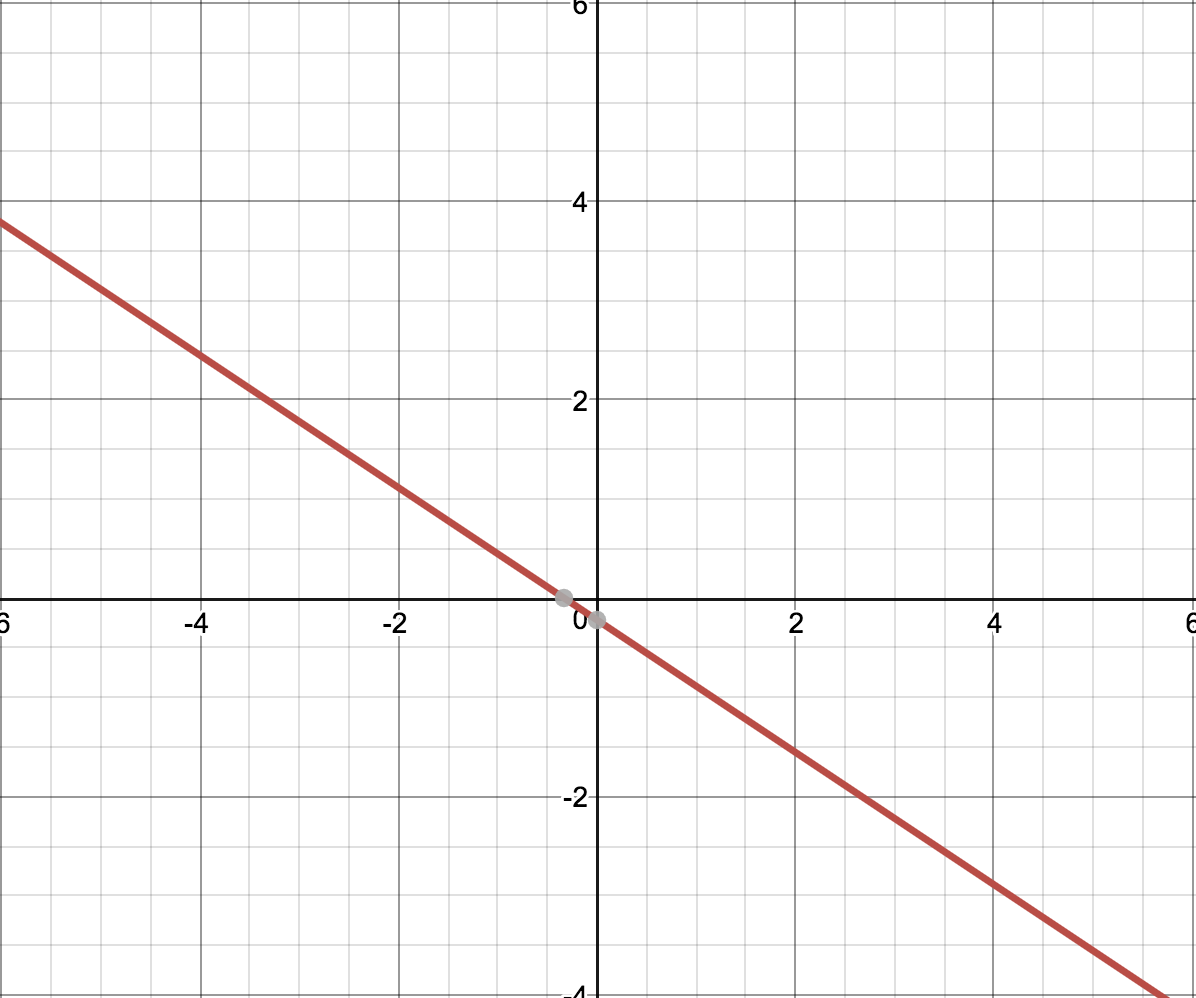
\includegraphics[width=0.5\textwidth]{c0.png}
        \caption{c = 0}
    \end{center}
\end{figure}
\begin{figure}[h!]
    \begin{center}
        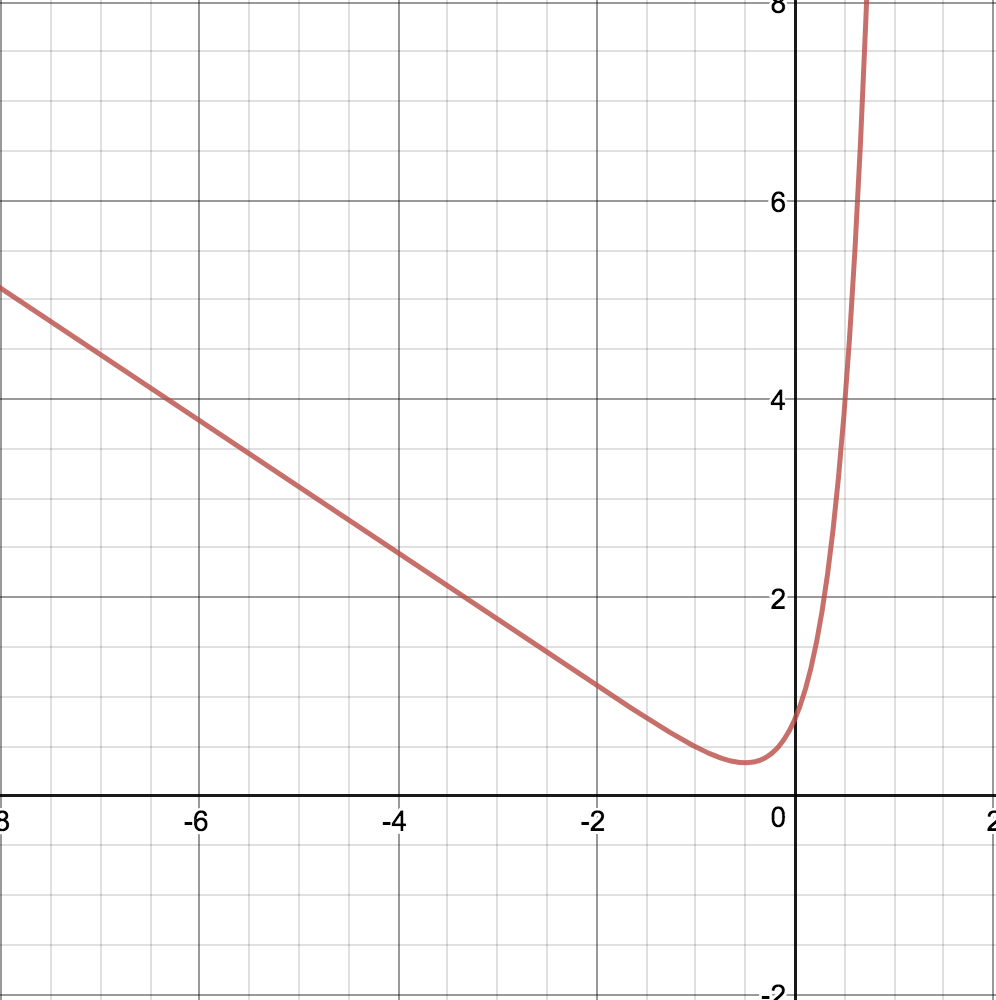
\includegraphics[width=0.5\textwidth]{c1.png}
        \caption{c = 1}
    \end{center}
\end{figure}

\begin{figure}[h!]
    \begin{center}
        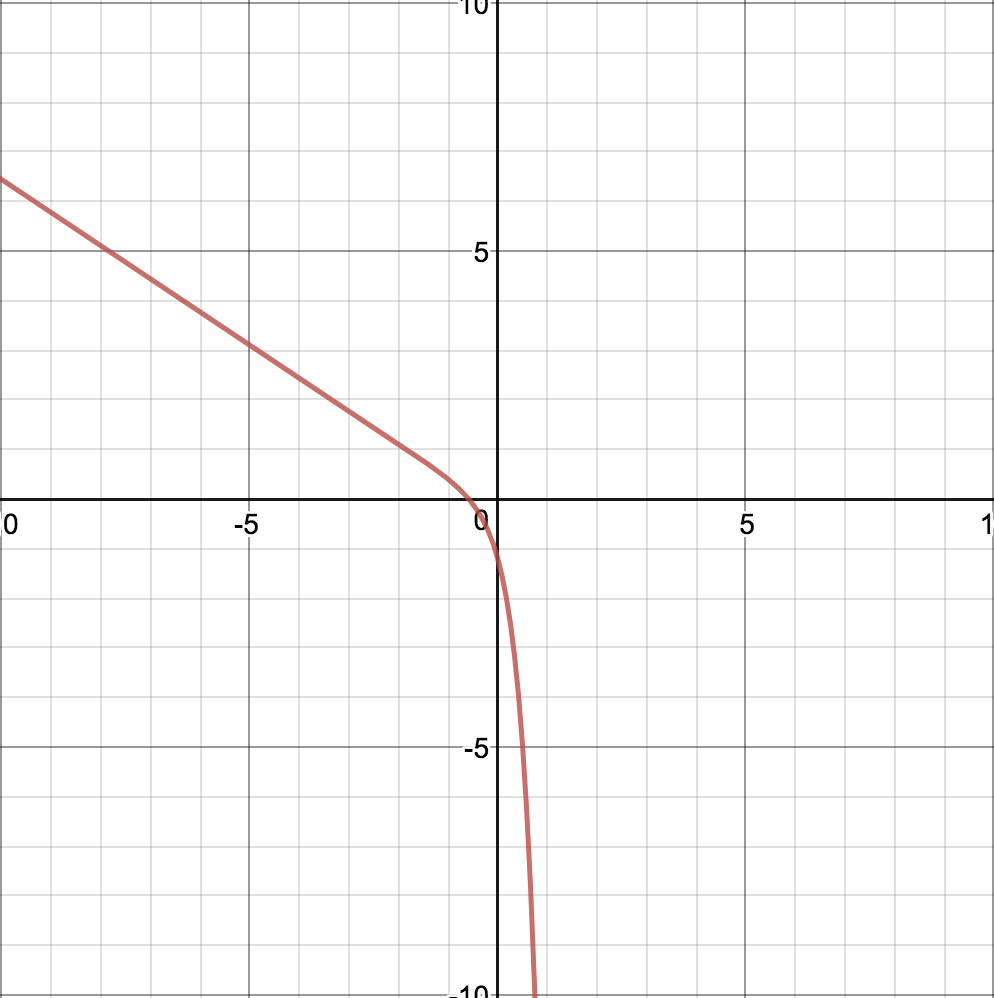
\includegraphics[width=0.5\textwidth]{c-1.png}
        \caption{c = -1}
    \end{center}
\end{figure}
\vspace{5000mm}
\clearpage
\newpage

\begin{center}
    {\LARGE 14th September Part 1}\\
\end{center}
\setcounter{subsection}{1}
\subsection{Linear ODE Revisited}
Consider $$\frac{dy}{dx} = p(x)y + q(x)$$
$$\frac{dy}{dx} - p(x)y = q(x) \;\;\;\;\;\;\;\;\;\;\;\text{Solution Set } S$$
$$\frac{dy}{dx} - p(x)y = 0 \;\;\;\;\;\;\;\;\;\;\;\text{Solution Set } \widetilde{S}$$

\textbf{Lemma 1:} If $y_1, y_2\; \epsilon\; \widetilde{S}$ then $c_1y_1 + c_2y_2\; \epsilon\; \widetilde{S}$, $c_1,\; c_2 \epsilon \R$ \\
\textit{Proof:} We know $\frac{dy}{dx} - p(x)y_1 = 0$ and $\frac{dy}{dx} - p(x)y_2 = 0$, what about $\frac{d}{dx}(c_1y_1 + c_2y_2) -p(x)(c_1y_1 + c_2y_2)$ On simplifying the last equation we get it's equal to zero \\\\
\textbf{Lemma 2:} Let $z_1,\;z_2\;\epsilon S$ then  $z_1,\;z_2\;\epsilon \widetilde{S}$\\
\textit{Proof:} We know $\frac{dz_1}{dy} - p(x)z_1 = q(x)$ and $\frac{dz_2}{dy} - p(x)z_2 = q(x)$, what about $\frac{d}{dx}(z_1-z_2) -p(x)(z_1-z_2) = 0$ On simplifying the last equation we get it's equal to zero \\\\
\textbf{Lemma 3:} Let $y_p\; \epsilon\; S$ (a particular solution), then $S\; =\; \{y+y_p:\; y\; \epsilon\; \widetilde{S}\}$
\textit{Eg: } $\frac{dy}{dx} -3y = 3x$
Consider  $\frac{dy}{dx} -3y = 0$, One solution is $y\equiv 0$ otherwise $\int\frac{dy}{y} = \int3dx$
$$\implies ln|y| = 3x + c \implies y = De^{3x}\;\;\;\;\;\;\;\; D \epsilon \R$$ Solution set of the associated homogeneous ODE is $\{De^3x: D\; \epsilon\; \R\}$
We need a $y_p$ - a special solution of the DE. We will guess this one. Let $$y_p = ax+b$$, $a$ and $b$ to be found.
$$\frac{dy_p}{dx} - 3y_p \equiv 2x \implies a -3(ax + b) \equiv 2x \implies a-3b - 3ax \equiv 2x$$
Comparing coefficients:
$$-3a = 2 \implies a = \frac{-2}{3}$$
$$a = 3b \implies b = \frac{-2}{9}$$
Thus $y_p = -\frac{2}{3}x - \frac{2}{9}$ and the complete solution set is $\{-\frac{2}{3}x - \frac{2}{9} + De^3x: D\; \epsilon\; \R\}$
\pagebreak
\subsection{Initial Value Problems}
When we solve a first order ODE we do not get a single function. We actually obtain a one parameter ($c$ - int constant) family of functions.\\
Often in practice we are provided with some extra information which allows us to choose one and only one of this family $i.e.$ the unique solution.\\
Often we have $x = x(t)$ and conditions at $t = 0$ and so the condition(s) of are referred to as initial condition.
The differential equation along with the initial condition together form an initial value problem

\begin{center}
    {\LARGE 14th September Part 2}\\
\end{center}

\paragraph{Aside Differentials}
$dx$ change in $x$, $dy$ change in $y$, leads to $dz$ change in $z$
$$z = H(x,y)$$
$$dz = \frac{\partial H}{\partial x}dx + \frac{\partial H}{\partial y} dy$$
But if we're on $z =\;\;\; constant \implies dz = 0 \implies z = c = H(x,\;y)$
$$0 = \frac{\partial H}{\partial x}dx + \frac{\partial H}{\partial y} dy \text{ [         implicit equation for } y]$$ and we can do something called implicit differentiation
$$\frac{\partial H}{\partial x} + \frac{\partial H}{\partial y} \frac{dy}{dx} = 0$$


\subsection{Exact $1^{st}$ order ODEs}
Suppose we have our $1^{st}$ order ODE $$\frac{dy}{dx} = F(x,y)$$. When we have to solve the ODE, we can always express the answer in the form $$G(x,y) = k$$ where k is a constant.

Our solution from earlier becomes: $$G(x,y) = \frac{y + \frac{2}{3}x + \frac{2}{9}}{e^{3x}}$$

If we differentiate this expression:
$$\frac{\partial G}{\partial x} + \frac{\partial G}{\partial y}\frac{dy}{dx} = 0$$
$$\implies \frac{dy}{dx} = -\frac{\frac{\partial G}{\partial x}}{ \frac{\partial G}{\partial y}}$$

Comparing the two $$\frac{dy}{dx} = F(x,y)$$ and $$\implies \frac{dy}{dx} = -\frac{\frac{\partial G}{\partial x}}{ \frac{\partial G}{\partial y}}$$

We must have, $$-\frac{\frac{\partial G}{\partial x}}{ \frac{\partial G}{\partial y}} = F(x,y)$$

There is some choice here:
$$\frac{\partial G}{\partial x} = m(x,y)F(x,y)$$
$$\frac{\partial G}{\partial y} = -m(x,y)$$
If we can find a $G(x,y)$ with $\frac{\partial G}{\partial x} = m(x,y)F(x,y)$ and
$\frac{\partial G}{\partial y} = -m(x,y)$. Then the solution is $G(x,y) = A$.

In practice we consider $\frac{dy}{dx} = F(x,y)$ is when teh function $F(x,y) = \frac{-M(x,y)}{N(x,y)}$, which we re-write as: $$M(x,y)dx + N(x,y)dy = 0$$
We want a solution of the following form $G(x,y) = c$
$$\frac{\partial G}{\partial x}dx + \frac{\partial G}{\partial y} dy = 0$$
We need         $$\frac{\partial G}{\partial x} = M(x,y)$$ and $$\frac{\partial G}{\partial y} = N(x,y)$$
\textit{How do we know whether these partial differential equations can be solved?}
If
$$\frac{\partial^2G}{\partial x \partial y} = \frac{\partial^2G}{\partial y \partial x}$$
Extending the earlier equations:
$$\frac{\partial }{\partial y}\frac{\partial G}{\partial x} = \frac{\partial M(x,y)}{\partial y} \equiv \frac{\partial }{\partial x}\frac{\partial G}{\partial y} = \frac{N(x,y)}{\partial x}$$

Given the ODE $mdx + Ndy = 0$ we say that the equation is exact to mean that the condition above is satisfied $\frac{N(x,y)}{\partial x} = \frac{\partial M(x,y)}{\partial y}$

\textit{Eg:}
$$
\frac{dy}{dx} = \frac{-1}{\frac{-(6y^2-x^2+3}{3x^2-3xy+2}}
$$
We re-write that as: $(3x^2-3xy+2)dx + (6y^2-x^2+3)dy = 0$\\
Is it possible that $\frac{\partial G}{\partial x} = 3x^2-2xy + 2 = M$ and $\frac{\partial G}{\partial y} = 6y^2 -x^2 + 3 = N$\\
We can solve this if $\frac{\partial^2G}{\partial x \partial y} = \frac{\partial^2G}{\partial y \partial x}$\\
$\frac{\partial M}{\partial y} = -2x$ and $\frac{\partial N}{\partial x} = -2x$
There is a solution, since this DE is exact\\\\
We want a function $G$ which $\frac{\partial G}{\partial x} = 3x^2 + 2xy + 2$
A solution is $G(x,y) = x^3 -x^2y + 2x$\\The most general solution is $G(x,y) = x^3 -x^2y + 2x + A(y)$ where $A(y)$ is a function of y\\\\
We also need $G$ to satisfy $\frac{\partial G}{\partial y} = 6y^2 -x^2 + 3$\\
A solution is $G = 2y^3 -x^2y + 3y$.\\ The most general solution is $G = 2y^3 -x^2y + 3y + B(x)$ where $B(x)$ for some function $B(x)$\\\\
Thus, the general solution of the DE is: $G(x,y) = x^3 + 2y^3 - x^2y + 2x + 3y + c$

\newpage

\begin{center}
    {\LARGE 18th September}\\
\end{center}
Last time we had the solution $G(x,y) = x^3 + 2y^3 - x^2y + 2x + 3y + k$\\
Solution is $G=c$, but we don't want two constants so we have to choose either of these:

$x^3 + 2y^3 - x^2y + 2x + 3y + k = 0$ or $x^3 + 2y^3 - x^2y + 2x + 3y = c$

Instead of remembering formulas remember:

$Mdx + Ndy = 0$ and that our solution for that is $\frac{\partial G}{\partial x}dx + \frac{\partial G}{\partial y}dy = 0$ and thus, $M=\frac{\partial G}{\partial x}$ and $N = \frac{\partial G}{\partial y}$.

And for a nice function $f$
$$\frac{\partial^2G}{\partial x \partial y} = \frac{\partial^2G}{\partial y \partial x} \implies \frac{\partial M}{\partial y} = \frac{\partial N}{\partial x}\;\;\;\;\;\;\;\;\;\;\;\; \text{Clairaut's theorem on equality of mixed partials}$$

\subsubsection{Why could the Clairaut's theorem on equality of mixed partials fail for a G}
$$xe^{xy} = c$$
Differentiating,
$$(e^{xy}+xye^{xy})dx + x^2e^{xy}dy = 0 \implies \frac{dy}{dx} = -\frac{e^{xy} + xye^{xy}}{x^2e^{xy}} \;\;\;\;\;\;\; xy \neq 0$$
And since $e^{xy} \neq 0$ then can we not factor it out of the equation
$$(1+xy)dx + x^2dy = 0$$
Now the question being whether this is exact?
Let $$M = 1+xy\;\;\;\;\;\;\;\;\;\;\; N = x^2$$
$$\;\;\frac{\partial M}{\partial y} = x\;\;\;\;\;\;\;\;\;\;\;\;\;\;\;\;\; \frac{\partial N}{\partial x} = 2x$$
This means that the equation earlier is not exact since there are not exactly the same functions.

Now we are in a situation that we need to find the missing function, and need to find what it is. It's called the Integration factor method
\subsection{Integration Factors}
Suppose we have to find a first order ODE that is not exact.\\
How de we proceed?\\
Solution: We multiply the ODE by an unknown function $I(x,y)$, called an integration factor. We try to make the new ODE exact
$$\text{i.e.} \;\;\; Mdx + Ndy = 0$$
And $M_y \not\equiv N_x \;\;\;\; \text{which is not exact, and we remedy by multiplying with I} \implies MIdx + NIdy = 0$\\
We want this to be exact  $(MI)_y \equiv (NI)_x$, which now imposes a restriction on $I$\\\\
Sadly we started from an ODE, but we moved to a PDE i.e. we are in a bigger mess now. Differentiating:
$$I\frac{\partial M}{\partial y} + M\frac{\partial I}{\partial y} \equiv I\frac{\partial N}{\partial x} + N\frac{\partial I}{\partial x} \;\;\;\;\;\;\;\;\;\;\;\; (**)$$
This is very hard to solve in general, however there are two special cases:\\
\textbf{Case 1:}
$I(x,y) = I(x)$ The PDE $(**)$ becomes
$$I\frac{\partial M}{\partial y} \equiv I\frac{\partial N}{\partial x} + N\frac{dI}{dx}$$

Collect all the terms in $I$ together,
$$\frac{1}{I}\frac{dI}{dx} = \frac{1}{N}(\frac{\partial M}{\partial y} - \frac{\partial N}{\partial x})$$
Since the LHS in the left, is just a function of $x$ only, then the RIHS must also be a function of $x$ only.\\
The RHS involves terms from the ODE, and we now have a test for an integration factor of the form $I = I(x)$

\textit{Eg:} = $\frac{dy}{dx} = -\frac{1+xy}{x^2}$, given $x^2 \neq 0$
$$(1+xy)dx + (x^2)dy$$
$$\implies M = 1+xy \implies M_y = x$$
$$\implies N = x^2 \implies N_x = 2x$$
Thus, $x \not\equiv 2x$, i.e. they are not identical, but they can be equal at $x = 0$
We examine $\frac{M_y - N_x}{N} = \frac{x-2x}{x^2} = -\frac{1}{x}$\\
Since is this a function of $x$ only,
\begin{itemize}
    \item There will be an integration factor for the DE of the form $I(x,y) = I(x)$
    \item $\frac{dlnI}{dx} = -\frac{1}{x}$, integration $ln(I) = ln|\frac{1}{x}|$ and one solution is $I(x) = x^{-1}$
\end{itemize}
Solution: $(1+xy)dx + x^2dy = 0$, multiplying by $I(x)$ we get $$(x^{-1} +y)dx + xdy = 0$$
Find $G(x,y)$ such that $G_x = x^{-1} + y \implies ln|x| + xy + H(y) = G$
and $G_y = x \implies xy + H(x) = G$\\
Therefore $G(x,y) = xy + ln|x|$ and the solution becomes: $G(x,y) = xy + ln|x| = c$\\
\end{document}
